\documentclass[a5paper]{article}
\usepackage[a5paper, top=8mm, bottom=8mm, left=8mm, right=8mm]{geometry}

\usepackage{polyglossia}
\setdefaultlanguage[babelshorthands=true]{russian}

\usepackage{fontspec}
\setmainfont{FreeSerif}
\newfontfamily{\russianfonttt}[Scale=0.7]{DejaVuSansMono}

\usepackage[hang,multiple]{footmisc}
\renewcommand{\footnotelayout}{\raggedright}

\PassOptionsToPackage{hyphens}{url}\usepackage[xetex,linktocpage=true,plainpages=false,pdfpagelabels=false]{hyperref}
\hypersetup{colorlinks=true, linkcolor=blue, citecolor=blue, filecolor=blue, urlcolor=blue, pdftitle=1, pdfauthor=, pdfsubject=, pdfkeywords=}

\usepackage{tabu}

\usepackage{indentfirst}
\usepackage{minted}
\usepackage[normalem]{ulem}
\usepackage{xcolor}
\usepackage{graphicx}

\newcommand{\attribution}[1] {
    \begin{flushright}\begin{scriptsize}\textcolor{gray}{#1}\end{scriptsize}\end{flushright}
}

\sloppy
\pagestyle{plain}

\title{Практика 7: архитектурная документация}
\author{}
\date{28.02.2022}

\begin{document}

\maketitle
\thispagestyle{empty}

\section{Архитектурная документация}

В этой лекции будет рассказано, что такое архитектурная документация и как именно её писать. Большая часть документации в реальной практике пишется довольно неформально, однако есть индустриальные стандарты (IEEE 1016-2009, ISO/IEC/IEEE 42010:2011, он же ГОСТ Р 57100-2016, плюс в какой-то степени семейство стандартов ГОСТ 19 --- ЕСПД). Знать их наизусть и свято следовать им не нужно (если только вы не работаете в оборонной промышленности или вообще на госзаказ), но, как обычно со стандартами, их писали умные люди, поэтому стоит иметь их в виду --- там по крайней мере написано, про что надо подумать. В этой лекции разберём IEEE 42010:2011 как самый свежий из действующих  (у него есть и русская версия, ГОСТ Р 57100-2016\footnote{ГОСТ Р 57100-2016, URL: \url{https://standartgost.ru/g/ГОСТ_Р_57100-2016} (дата обращения: 26.01.2022).}, но она просто местами странный перевод стандарта ISO, так что лучше смотреть оригинал), и IEEE 1016-2009, как пример конкретных рекомендаций по структуре документа.

Но для начала --- о том, что такое вообще архитектурная документация и зачем она нужна. Вообще, архитектурная документация --- это основной продукт работы архитектора, именно архитектурный документ фиксирует архитектуру. Так что бесполезно рассказывать целый курс об архитектуре, не рассказав, а что же, собственно, и как в архитектурный документ надо писать.

Архитектурная документация --- \emph{не} набор UML-диаграмм, хотя рекомендуется активно их использовать. Документ должен представлять, возможно более полно и однозначно, основные архитектурные решения, и, что главное, их объяснять. 

Есть известный организационный антипаттерн <<Architecture By Implication>> --- когда команда считает, что не стоит явно специфицировать архитектуру, ведь подобные задачи уже решались в прошлом, к тому же и так понятно, что надо делать, а архитектурная документация требует времени для разработки и сил для сопровождения. Иногда это проходит без последствий, но чаще --- оказывается, что с того момента, как команда делала подобную систему, успели выйти новые библиотеки и технологии, или предметная область немного другая, или в команду пришёл новый человек и он без идей, как задачу решали в прошлый раз. И оказывается, что на последних этапах разработки команду ждут неприятные сюрпризы, из-за которых, возможно, вообще всё надо будет переделывать. 

Хорошая архитектурная документация (а также практика её всё-таки писать хоть в каком-то виде до начала реализации) как раз и решает такую проблему. Индустриальная практика говорит, что хороша архитектурная документация может сократить затраты на кодирование в разы. Поэтому, чаще всего имеет смысл всё-таки потратить время на создание и описание архитектуры, и оно потом вернётся с процентами при реализации. Для студентов есть и более прагматичные причины создания архитектурной документации --- её можно включать с минимальными правками в тексты отчётов по практикам/НИР/ВКР, которые в любом случае надо будет писать, и лучше писать структурированно и в соответствии с хорошими практиками.

Как уже говорилось, в индустриальной практике архитектурная документация наличествует в основном в неформальном виде. Чаще всего это страницы в корпоративном вики, набор .md-файлов в репозитории и т.п. Проекты с открытым исходным кодом обычно вообще не заморачиваются такими вещами, поскольку участники программируют в своё удовольствие и не очень горят желанием писать тексты. Тем не менее какая-то документация по архитектуре есть практически во всех проектах, известных автору. Представление о стандартах может помочь в написании неформальных архитектурных описаний --- стандарт можно рассматривать как некий чеклист, позволяющий проверить, что обо всём важном подумали, и что всё написанное служит какой-то осмысленной цели. 

Кстати, в игровой индустрии есть ещё понятие Game Design Document, и если будете искать в интернете про Design Document, то с большой вероятностью найдёте именно про него. Это немного не то. То есть типичный Game Design Document служит тем же целям, что и архитектурная документация --- подумать о всех важных вещах заранее --- и довольно схож по структуре, но в Game Design Document существенно большее внимание уделяется нетехническим вещам. Там больше про геймплей, игровые механики и т.п.

\subsection{Общие рекомендации}

Самое сложное при написании архитектурной документации --- это то, что она должна быть достаточно подробной, чтобы при программировании не требовалось принимать никаких важных архитектурных решений, и вместе с тем, достаточно краткой, чтобы её кто-нибудь прочитал. Как и архитектура вообще, написание архитектурной документации --- это искусство, и начинающим архитекторам бывает сложно понять, что является важным архитектурным решением, а что нет. Так что написать хороший архитектурный документ сложно. Однако сообщество сходится на том, что даже плохой архитектурный документ лучше, чем никакого.

Чтобы архитектурный документ был обозримым, в нём активно используются \emph{точки зрения} --- описания, предназначенные для разных целевых аудиторий и описывающих разные аспекты архитектуры. Для руководства в начале документа обычно краткая выжимка (одна-две страницы) о назначении и смысле существования системы, для технических людей подробное описание того, как всё устроено, для обслуживающего персонала (админов и т.п. --- отдельные разделы про то, как это всё настраивать) и т.д. Впрочем, и для одной целевой аудитории используются разные точки зрения, например, программистам может быть интересна и статическая структура системы, и поведение во время выполнения, и схема базы данных. Это сродни архитектуре здания, где есть отдельно поэтажный план, отдельно план проводки, отдельно план канализации.

Продолжая аналогию с архитектурой зданий, для представления разных точек зрения используются разные <<чертежи>> --- визуальные нотации. Разные точки зрения доносятся до читателя с помощью разных визуальных языков, специально заточенных под эти точки зрения. В основном это UML, поскольку он стандартный, но другие языки тоже часто применяются (ER-диаграммы, например). Ещё раз обращаю внимание, что диаграммы не описывают архитектуру, а только иллюстрируют архитектурное описание, так что основную мысль надо доносить всё-таки текстом.

Хорошая архитектурная документация должна не только документировать принятые решения, но и:

\begin{itemize}
    \item альтернативы --- из чего и по каким критериям выбирали, и почему выбрали то, что выбрали. Это важно для дальнейшего сопровождения системы --- при изменении требований или даже просто рефакторинге, возможно, захочется что-то поменять в архитектуре, и не хотелось бы выполнять работу по анализу с нуля (возможно, не один раз). Например, в команду пришёл новый разработчик, и говорит, что всю жизнь использовал фреймворк А, давайте всё на нём перепишем. Если в архитектурной документации написано, почему вы используете фреймворк Б, и что вы рассматривали А, но отказались по таким-то причинам, это может сэкономить массу усилий. А вот если А не упоминается (например, вышел после того, как вы искали фреймворки), то, может, как раз стоит попробовать.
    \begin{itemize}
        \item Однако надо обязательно чётко формулировать, что в итоге решили. Есть архитектурный антипаттерн <<Cover your assets>> (если вы понимаете, о чём я), когда документация пишется в виде <<а можно вот так, а можно ещё вот так>>. Тогда все ошибки в архитектуре можно свалить на разработчиков, которых можно обвинить в том, что они неправильно поняли, какую из альтернатив надо реализовать. Ну и вообще, архитектору не надо брать ответственность за выбор, очень удобно (вот только полностью обесценивает архитектора для команды).
    \end{itemize}
    \item Там, где это важно, опишите также преимущества и риски, связанные с принятым решением. Причём, по возможности объективно --- ваша цель не продать решение, а сохранить свои мысли и идеи на случай, если ситуация изменится (например, поменяются требования) и решение надо будет пересматривать. Риски в духе <<а если вдруг надо будет сделать вот так, то в нашей архитектуре это нормально не сделать>> вполне ок и могут сэкономить кучу времени в будущем. Хотя, конечно, всё не предусмотришь, и придумывать кучу надуманных проблем для своего решения тоже не надо.
    \item Надо пояснить связь решений с требованиями. Некоторые нотации (например, SysML) предполагают, что это будет делаться формально, но чаще просто текстом поясняют, что компонент такой-то реализует функциональные требования такие-то, или решение такое-то было принято, чтобы удовлетворить тому-то и тому-то. Опять-таки, требования имеют свойство меняться, и \emph{трассируемость} требований сильно поможет при сопровождении архитектуры.
\end{itemize}

Важно также следить за \emph{полнотой} и \emph{консистентностью} архитектурного описания. Полнота означает, что на все важные для архитектуры вопросы в документации есть ответ, все требования покрыты и все интересы стейкхолдеров учтены. Консистентность означает отсутствие внутренних противоречий в документации.

\section{Стандарт ISO/IEC/IEEE 42010:2011, архитектурное описание}

Мир стандартов устроен довольно странно --- стандарт ISO/IEC/IEEE 42010:2011 ``Architecture description'' стандартизует не структуру архитектурного описания, а его основные концепции и общие требования, так что может показаться довольно болтологическим. В каком-то смысле это <<метастандарт>> в том смысле, что он больше полезен авторам архитектурных фреймворков или корпоративных шаблонов, по которым уже потом будет писаться архитектурная документация. Однако он содержит ряд интересных мыслей, поэтому сначала рассмотрим именно его. Дальнейшее изложение, правда, является вольным пересказом идей из стандарта и не претендует на нормативность. Если кому важны конкретные формулировки, определения и т.п., найдите оригинальный стандарт, благо он есть в открытом доступе, размером всего 46 страниц и с картинками.

\subsection{Концептуальная модель архитектурного описания}

Вот так стандарт вводит основные элементы контекста, в котором пишется архитектурная документация:

\begin{center}
    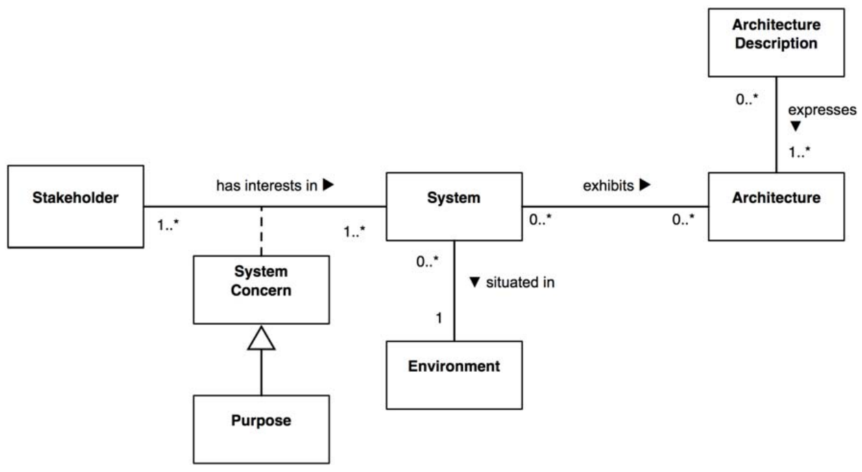
\includegraphics[width=0.9\textwidth]{ieee42010Context.png}
\end{center}

Как видно, модель предметной области архитектурной документации --- это диаграмма классов UML (потому что стандарты по архитектурной документации пишут люди, умеющие писать архитектурную документацию, очевидно). Что входит в контекст:

\begin{itemize}
    \item System --- документируемая система (стандарт намеренно не определяет понятие <<система>>, позволяя рассматривать как программные, так и программно-аппаратные системы, или даже системы с человеческим участием);
    \item у системы есть некоторая архитектура (Architecture), даже если она пока явно не зафиксирована;
    \begin{itemize}
        \item обратите внимание на множественность ассоциаций --- стандарт рассуждает по поводу того, что у одной системы может быть несколько разных архитектурных описаний (которые рассматриваются как разные архитектуры), и одна архитектура может покрывать несколько систем (типовая архитектура в компании, например);
    \end{itemize}
    \item архитектурное описание (Architecture Description) --- то самое, про что стандарт; оно, как подсказывает здравый смысл, описывает архитектуру;
    \item система существует в некотором окружении (Environment);
    \item и удовлетворяет интересам некоторых стейкхолдеров (Stakeholder) --- заинтересованных лиц в самом общем смысле, от пользователей до программистов;
    \begin{itemize}
        \item эти интересы выражаются концепцией System Concern (несколько неуклюже переведённым в ГОСТ как <<системный интерес>>), из которых самый важный --- это цель существования системы (Purpose).
    \end{itemize}
\end{itemize}

Более содержательна модель самого архитектурного описания:

\begin{center}
    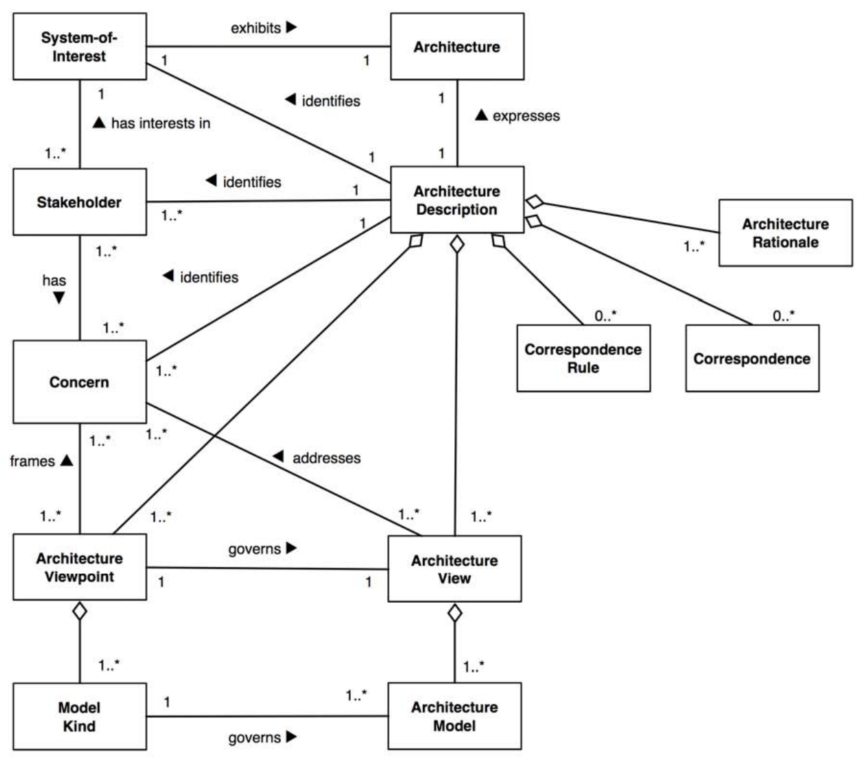
\includegraphics[width=0.9\textwidth]{ieee42010ArchitectureDescription.png}
\end{center}

Из нового тут самое важное --- это ключевые для стандартов 42010 и 1016 понятия <<Architecture View>> и <<Architecture Viewpoint>>. Архитектурный вид --- это срез архитектуры системы согласно какой-то точке зрения (которую регламентирует Architecture Viewpoint). Например, статическое представление системы, её развёртывание, динамическое поведение в виде конечного автомата и т.д. Architecture Viewpoint описывает правила, по которым строятся Architecture View и какие Concern-ы должны покрывать --- например, UML является готовым набором из 14 Architecture Viewpoint-ов. Сама содержательная часть архитектурного описания --- это как раз набор Architecture View, с отсылками к соответствующим им Architecture Viewpoint-ам (или с подробным описанием Viewpoint-а прямо в архитектурной документации, стандарт это предполагает, но в реальной жизни никто не заморачивается).

Architecture View состоит, в свою очередь, из набора моделей. Каждая из которых соответствует типу модели (как правило, задаваемому \emph{метамоделью} визуального языка, но модели бывают не только визуальные). В Architecture Viewpoint может входить несколько видов моделей (например, статическая структура системы может описываться совместно диаграммами компонентов и диаграммами классов UML), в архитектурный вид, соответственно, несколько моделей (может, одного вида, может, нескольких). 

Причём, самое интересное, что стандарт IEEE 42010:2011, в отличие от IEEE 1016-2009, никак не регламентирует Architecture Viewpoint-ы, то есть \emph{никак} не регламентирует то, из чего именно должна состоять архитектурная документация. Это кажется удивительным, но сделано с умом --- стандарт признаёт существование \emph{архитектурных фреймворков} и говорит, что как именно описывать архитектуру --- это их дело. В самом стандарте приводятся как примеры фреймворки Zachman’s information systems architecture framework, UK Ministry of Defence Architecture Framework, The Open Group’s Architecture Framework (TOGAF), Kruchten’s ``4+1'' view model, Siemens’ 4 views method, Reference Model for Open Distributed Processing (RM-ODP), Generalized Enterprise Reference Architecture (GERA). Стандарт поощряет использование предметно-ориентированных фреймворков и референсных архитектур, даже создание своих внутрикорпоративных архитектурных фреймворков. Приводится даже модель типичного архитектурного фреймворка (которая достаточно размыта, чтобы под неё подходили все перечисленные):

\begin{center}
    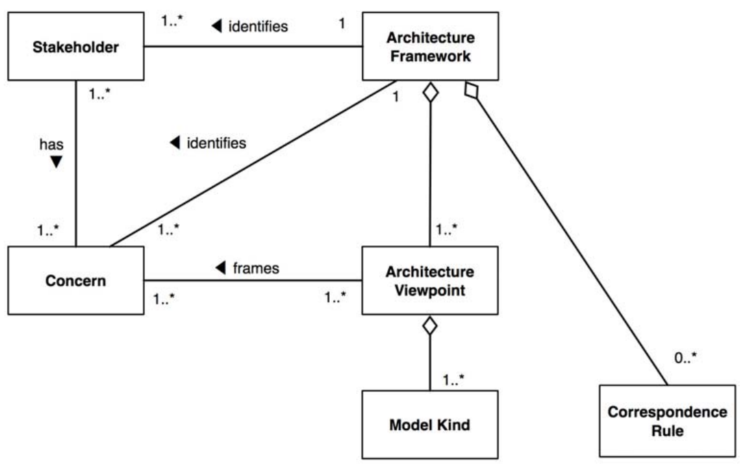
\includegraphics[width=0.8\textwidth]{ieee42010ArchitectureFramework.png}
\end{center}

Тут по сравнению с предыдущей диаграммой ничего нового нет, но второй раз встречается Correspondence Rule, которое пока никак не пояснялось. Итак, Correspondence Rule --- это правило, по которому элементы архитектуры должны быть связаны друг с другом. Ему может соответствовать несколько Correspondence --- конкретных экземпляров взаимосвязей между элементами. Например, то, что каждый случай использования должен иметь хоть один компонент или класс, который его реализует --- это Correspondence Rule, а отношение <<trace>> между конкретным случаем использования с соответствующей диаграммы и конкретным классом с диаграммы классов --- это Correspondence, ему соответствующий.

Ещё стандарт обращает внимание на то, что основная роль архитектуры --- документировать \emph{и объяснять} архитектурные решения, поэтому понятия архитектурного решения и объяснения удостоились собственной модели:

\begin{center}
    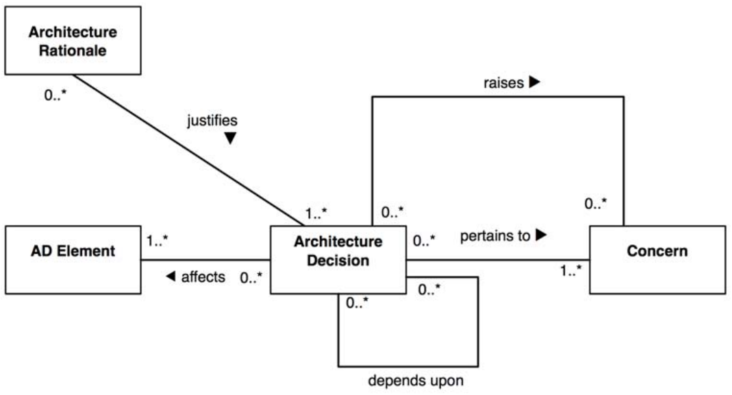
\includegraphics[width=0.8\textwidth]{ieee42010Decision.png}
\end{center}

AD Element тут --- это Architecture Description Element, то есть по сути любой элемент архитектурного описания, включая нестандартизованные элементы View. На них оказывает влияние Architecture Decision, которое в свою очередь объясняет Rationale. При этом Architecture Decision --- это всегда реакция на какой-то Concern (интерес стейкхолдера), и при этом может само формулировать новые Concern-ы. И, конечно, Architecture Decision могут быть связаны друг с другом зависимостями.

\subsection{Архитектурная документация}

Как уже говорилось, стандарт особо не регламентирует конкретный состав архитектурного документа, но некоторые требования всё-таки предъявляет. Вот что должно включаться в соответствующую стандарту архитектурную документацию.

\begin{itemize}
    \item Общая информация о документе и краткая информация о проектируемой системе --- где-то в начале должна быть идентифицирована описываемая система (то есть о чём вообще речь), и при необходимости предоставлена служебная информация типа авторов, даты, номера ревизии, глоссария.
    \item Должны быть описаны стейкхолдеры и их интересы. При этом требуется рассмотреть следующих стейкхолдеров и включить в документацию, если они релевантны:
        \begin{itemize}
            \item пользователей;
            \item операторов системы;
            \item тех, кто систему будет приобретать;
            \item тех, кто системой будет владеть;
            \item поставщиков системы;
            \item разработчиков системы;
            \item <<строителей>> системы --- видимо, людей, отвечающих за сборку и CI/CD, если речь идёт о программной системе, и всё становится более интересным, если система с физическими компонентами и людьми;
            \item ответственных за сопровождение системы.
        \end{itemize}
        При этом типичные интересы включают в себя (опять-таки, стандарт \emph{требует их рассмотреть} (используется глагол <<shall>>, означающий нормативное требование для соответствия стандарту), но не требует включать):
        \begin{itemize}
            \item назначение системы;
            \item насколько архитектура подходит для достижения целей существования системы;
            \item выполнимость разработки\footnote{В стандарте используется более общий термин <<constructing>>, который в ГОСТ 57100-2016 переведён как <<конструирование>>, но для программных систем это звучит странно --- напомним, что IEEE 42010 программными системами не ограничивается, зато ими ограничивается этот курс.} и развёртывания системы;
            \item потенциальные риски и влияние системы на стейкхолдеров\footnote{Кстати, в ГОСТ приводится правильный перевод <<заинтересованные стороны>>, но мы используем жаргонизм, чтобы избежать канцелярита.} на всех этапах её жизненного цикла.
            \item сопровождаемость и расширяемость (и вообще способность к эволюции) системы.
        \end{itemize}
    \item Определение каждой архитектурной точки зрения, используемой далее. Каждое соображение из пункта выше, которое включается в архитектурное описание, должно быть покрыто хотя бы одной точкой зрения. На практике полные определения никто не вставляет, все ссылаются на готовые стандарты/фреймворки (в частности, UML).
    \item Архитектурные виды --- та самая содержательная часть документа, на которую приходится процентов 90 его объёма. Каждой точке зрения из пункта выше должен соответствовать ровно один архитектурный вид (который, в свою очередь, может состоять из многих диаграмм и текстовых описаний).
        \begin{itemize}
            \item Что важно, \emph{каждый} архитектурный вид должен описывать \emph{всю} систему со своей точки зрения. То есть вы не можете нарисовать диаграмму состояний для одного компонента, а для другого, у которого тоже есть нетривиальная логика состояний и переходов, не рисовать. Этим стандарт надеется обеспечить полноту и консистентность документации. Однако обратите внимание, что каждый вид рассматривает только тот аспект архитектуры, который ему интересен, поэтому если у вас только один компонент имеет автомат внутри, то для всех остальных тривиальные автоматы из одного состояния рисовать не надо.
            \item Ещё каждый вид должен явно выписывать все известные проблемы, включая открытые вопросы, нарушения ограничений (включая нарушения Correspondence Rules) или отклонения от нотации. Стандарт допускает неконсистентность (поскольку справедливо говорит, что взять и сразу сделать всё хорошо и правильно, как правило, невозможно или слишком дорого). Однако требует её явно документировать, чтобы потом не забыть.
            \item Вид состоит из моделей, но стандарт не требует, чтобы модель относилась к одному определённому виду --- разрешается шарить модели между видами, во избежание копипаста. Что за модели, как они создаются и как используются, стандарт не специфицирует.
        \end{itemize}
    \item Отношения между элементами архитектуры --- Correspondences и Correspondence Rules, о которых шла речь выше. Вплоть до рисования табличек с соответствием элементов модели. Никогда не видел такого на практике.
    \item Обоснование архитектуры (Rationale) --- для каждой архитектурной точки зрения и для каждого ключевого архитектурного решения. В стандарте приводится длинный список того, как понять, какие решения ключевые и что надо обосновывать, но это в целом должно быть интуитивно понятно. Стандарт, однако, обращает внимание на важную вещь --- каждое решение должно быть чётко сформулировано (чтобы не было <<а можно так, а можно сяк>>).
    
    Крайне желательно также описывать рассмотренные альтернативы и объяснять, почему было выбрано то, что выбрано.
    
    На самом деле всё это приводится обычно не отдельным пунктом документа, а прямо внутри описания архитектурных видов --- документируем решения и тут же обосновываем их. Стандарт не против, он предъявляет требования только к содержанию документа, а не к его структуре.
\end{itemize}

\section{Стандарт IEEE 1016-2009, Software Design Description}

Стандарт IEEE 1016-2009 мы тоже кратко рассмотрим, хоть он и неактивен с 2020 года, и во многом повторяет IEEE 42010. Нужен он нам потому, что он гораздо более специфичен в плане содержания архитектурной документации (из-за этого же, видимо, и отменён --- он пытается конкурировать с архитектурными фреймворками). В частности, в нём прописывается структура документа и выделяются архитектурные виды, которые надо рассмотреть, даже с рекомендациями относительно подходящих визуальных нотаций. Это неплохая отправная точка, и в этом курсе рекомендуется использовать его, если нет причин использовать какой-то более специфичный архитектурный фреймворк. <<Настоящих>> архитектурных фреймворков много, они, как правило, заточены под конкретную область применения и довольно громоздки, поэтому тут не рассматриваются.

\subsection{IEEE 1016-2009, концептуальная модель}

Модель архитектурного документа в IEEE 1016-2009 концептуально похожа на рассмотренную выше:

\begin{center}
    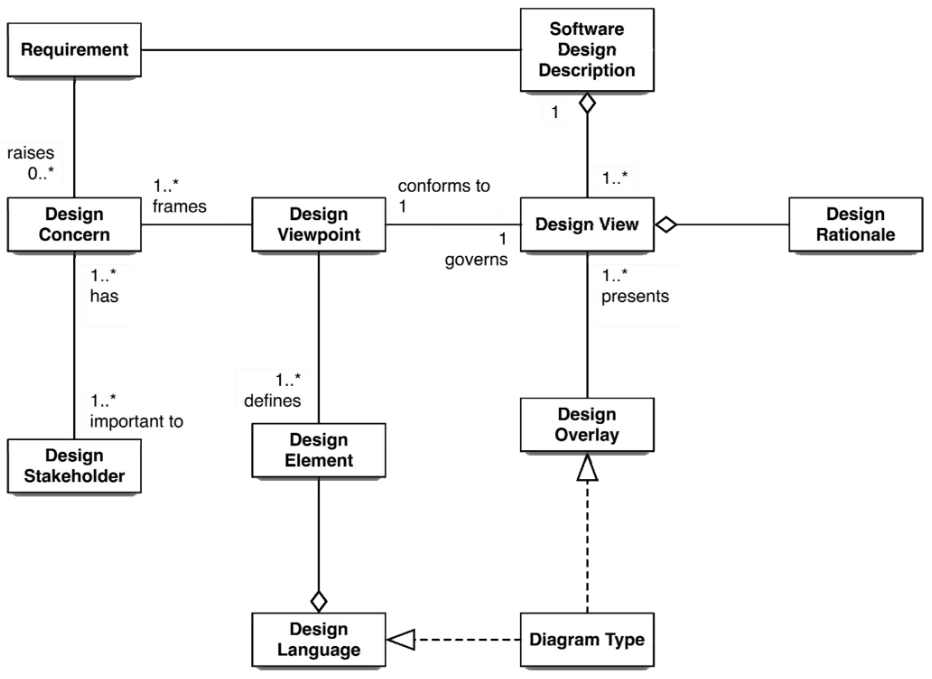
\includegraphics[width=0.95\textwidth]{ieee1016Concepts.png}
\end{center}

Обратите внимание, в этом стандарте тоже используется UML для моделирования документа.

Здесь также ключевыми концепциями являются Design View и Design Viewpoint, которые играют точно такую же роль, как аналогичные понятия в IEEE 42010. Единственное, что IEEE 1016 более ориентирован именно на архитектурные виды --- например, Rationale является свойством вида, а не архитектурного описания в целом, а Design Concern привязан к Viewpoint-у. Новым понятием является Design Overlay --- это уточнение View с, возможно, другой нотацией и немного другой точкой зрения на вещи, но в общем ключе Viewpoint-а. Viewpoint-ы определяют Design Element-ы, из экземпляров которых должны состоять View-ы, Design Element-ы принадлежат некоему языку (например, UML). Сами Design Element-ы --- это либо сущность с атрибутами, либо отношение между сущностями, либо ограничение:

\begin{center}
    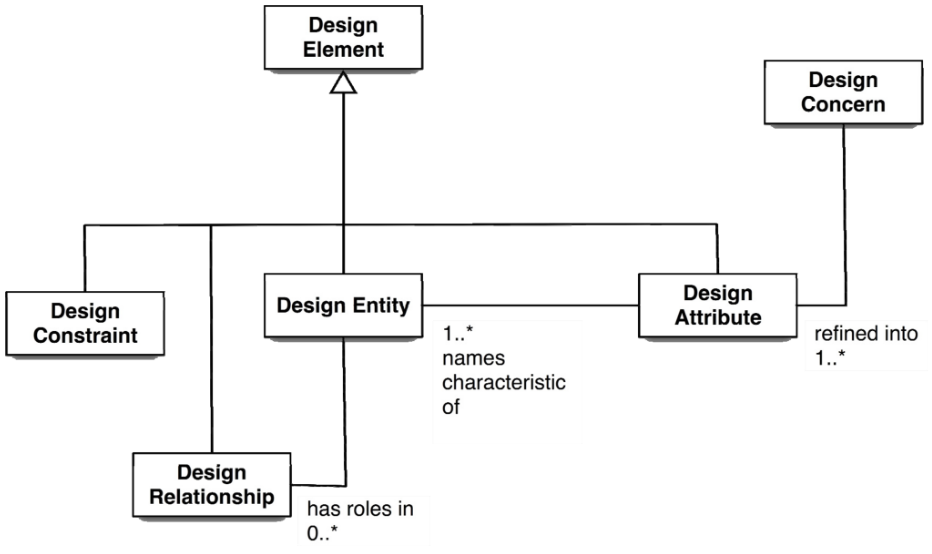
\includegraphics[width=0.8\textwidth]{ieee1016ArchitectureElements.png}
\end{center}

\subsection{IEEE 1016-2009, структура документа}

IEEE 1016-2009 предполагает конкретную структуру архитектурного документа.

\begin{itemize}
    \item Начинаться он должен с различной служебной информации (название, автор, дата, номер ревизии и т.д. и т.п., это стандарт не специфицирует, оставляя на откуп внутрикорпоративным правилам).
    \item Затем следует раздел <<Общие сведения о системе>>, состоящий (концептуально) из:
        \begin{itemize}
            \item описания назначения системы (один абзац текста, что за система и для чего она вообще);
            \item описания границ системы (Scope) --- чем система является, а чем нет (чтобы избежать проблемы <<feature creep>>, когда постепенным добавлением фич система превращается в умеющего всё монстра);
            \item краткого описания контекста, в котором система будет работать --- с какими внешними системами взаимодействует, куда развёртывается и т.п. (обратите внимание, это только самая общая информация, для деталей есть отдельные виды).
        \end{itemize}
    \item Затем идут Architectural drivers (за отсутствием адекватного перевода будем довольствоваться англоязычным термином) --- это ключевые требования, определяющие архитектуру. То, что должно оказывать наибольшее влияние на архитектуру системы и в большой степени её определяет. Они бывают:
        \begin{itemize}
            \item техническими ограничениями --- например, если вы пишете под iOS, это навязывает ряд ограничений в выборе технологий и даже архитектуры приложения;
            \item бизнес-ограничениями --- если через две недели демо, архитектура у системы будет совсем не такая, как если сдача проекта через три года;
            \item качественные характеристики системы --- сопровождаемость, расширяемость и т.п. Часто они конфликтуют друг с другом (например, погоня за скоростью работы может нанести серьёзный ущерб сопровождаемости). И именно качественные характеристики имеют решающее влияние на архитектуру. Если нужна максимальная производительность, будут использоваться совершенно другие архитектурные стили, языки и технологии, чем если нужна максимальная сопровождаемость или минимальный time-to-market.
            \item Ключевые функциональные требования тоже, безусловно, являются архитектурными драйверами, но только ключевые. Какие именно поля есть на форме --- абсолютно всё равно с точки зрения архитектуры, а вот функциональные требования, влекущие, например, распределённость приложения (например, коллаборативная работа над документом) --- критичны.
        \end{itemize}
    \item Дальше идут архитектурные виды, про которые подробнее дальше. Столько, сколько считает нужным архитектор, и таких типов, какие архитектор выбрал как наиболее полезные для описания архитектуры конкретной системы. Важно, правда, что каждый вид должен быть экземпляром некоторого Viewpoint-а. Стандарт не требует его явно определять, но должно быть понятно, о чём идёт речь --- например, диаграммы, <<напоминающие UML>>, использовать нельзя. Есть Viewpoint-ы, определяемые в UML, и тогда UML надо строго следовать. Если хочется свою нотацию, извольте её формально определить (лучше в отдельном документе).
    \item Rationale --- причины принятых решений, за/против, альтернативы. Вообще, всё это приводится в деталях при описании каждого View, в конце документа только summary. Это нужно, чтобы при изменении требований/ограничений/контекста проекта быстро пробежаться по аргументации и понять, какие аргументы уже неприменимы.
\end{itemize}

\subsection{IEEE 1016-2009, точки зрения и виды}

IEEE 1016 выделяет аж 12 точек зрения на систему. 

\begin{itemize}
    \item Контекст  --- описывает, что система должна делать, фиксирует окружение системы. Состоит из сервисов и акторов, которые могут быть связаны информационными потоками. Система представляет собой <<чёрный ящик>>, в том смысле что никак в этом виде не детализируется. Это корень иерархии уточняющих дизайн системы видов, стартовая точка при проектировании системы. Обычно описывается с помощью диаграмм активностей UML, IDEF0 (SADT). Также может быть определён Deployment overlay, показывающий развёртывание системы. Впрочем, если система сильно распределённая или аппаратное обеспечение --- часть разработки, Deployment выносится в отдельный вид.
    
    Основные интересы (concerns), покрываемые этим видом --- ключевые функциональные требования, роли пользователей системы, границы (scope) системы. 
    
    \item Композиция --- описывает крупные части системы и их предназначение. Предназначен для локализации и распределения функциональности системы по её структурным элементам, impact analysis-а, облегчения переиспользования (в том числе, покупки компонентов), оценки, планирования, управления проектом, определения необходимой инструментальной поддержки (репозитории, трекер и т.д.). Обычно описывается с помощью диаграмм компонентов UML, IDEF0, Structure Chart.
    \item Логическая структура --- структура системы в терминах классов, интерфейсов и отношений между ними. Также применяются и диаграммы объектов (хотя они относятся ко времени выполнения) --- для иллюстрации структуры классов. Типичные языки --- диаграммы классов UML, диаграммы объектов UML.
    
    Основные интересы --- разработка и переиспользование (часто переиспользование внутреннее, то есть переиспользование кода внутри проекта, хотя возможны и варианты закупки готовых компонентов).
    
    \item Зависимости ---  определяет связи по данным между элементами: разделяемая между элементами информация, порядок выполнения и т.д. Необходим для анализа изменений, идентификации узких мест производительности, планирования, интеграционного тестирования. Типичные языки --- диаграммы компонентов UML, диаграммы пакетов UML.
    
    \item Информационная структура --- определяет персистентные данные в системе (информация, которую требуется хранить, схема БД, доступ к данным). Типичные языки --- диаграммы классов UML, IDEF1x, ER.
    
    Для информационных систем это один из первых разрабатываемых видов, и он может быть определяющим для всей архитектуры системы.
    
    \item Использование шаблонов --- документирование использования локальных паттернов проектирования с целью поддержать переиспользование не только кода, но и хороших идей, и архитектурных стилей. Типичные языки --- диаграммы классов UML, диаграммы пакетов UML, диаграммы коллабораций UML.
    
    \item Интерфейсы --- специфицирует информацию о внешних и внутренних интерфейсах, не прописанную явно в требованиях. Пользовательский интерфейс рассматривается отдельным видом в рамках этой точки зрения. Типичные языки --- IDL, диаграммы компонентов UML, макеты пользовательского интерфейса, неформальные описания сценариев использования. Почему авторы стандарта не разделяют пользовательский и программный интерфейс, непонятно (да, и то и другое --- интерфейс, точка взаимодействия системы с внешним миром, но используются совершенно разные подходы и нотации).
    
    Интересы, покрываемые этим видом --- договорённости о конкретных схемах взаимодействия компонентов, что позволяет разрабатывать и тестировать компоненты независимо, и потом без проблем (ну, в большей или меньшей степени) собрать готовую систему. Макеты пользовательского интерфейса также позволяют распараллелить разработку бэкенда и работу дизайнеров/фронтенд-программистов.
    
    Это один из немногих видов, где текстовые языки описания программных интерфейсов (те самые IDL --- например, gRPC, Apache Thrift) предпочтительнее визуальных. А вместо языков использования пользовательских интерфейсов используются вообще неформальные рисунки.
    
    \item Структура системы --- рекурсивное описание внутренней структуры компонентов системы. Типичные языки --- диаграммы композитных структур UML, диаграммы классов UML, диаграммы пакетов UML. Вид, тоже предназначенный в первую очередь для программистов и архитекторов.
    
    \item Взаимодействия --- описывает взаимодействие между сущностями: почему, когда, как и на каком уровне выполняется взаимодействие. Типичные языки --- диаграммы композитных структур UML, диаграммы взаимодействия UML, диаграммы последовательностей UML.
    
    Интересы --- распределение ответственностей между участниками взаимодействия, определение протоколов взаимодействия.
    
    \item Динамика состояний --- описание состояний и правил переходов между состояниями в реактивных системах. Типичные языки --- диаграммы конечных автоматов UML, диаграммы Харела, сети Петри.
    
    Интересы --- поведение системы, включая внутренние состояния, события и логику переходов. Поскольку языки, описывающие машины состояний, имеют исполнимую семантику, этот вид допускает ещё и некую верификацию и моделирование работы системы. Правда, далеко не все системы можно содержательно представить в виде конечных автоматов, так что вид весьма ситуационный.
    
    \item Алгоритмы --- описывает в деталях поведение каждой сущности, логику работы методов. Типичные языки --- диаграммы активностей UML, псевдокод, настоящие языки программирования. Нужен этот вид для  анализа эффективности работы программы, помощи в реализации и юнит-тестировании. Ещё один вид, где применяются прежде всего текстовые языки. При этом главное --- не увлекаться, архитектура не должна отнимать хлеб у программистов. Описывать надо только ключевые алгоритмы системы, и только если они нетривиальны.
    
    \item Ресурсы --- описывает использование внешних ресурсов (как правило, аппаратных или третьесторонних сервисов). Нужно это прежде всего для анализа эффективности работы системы и требований к аппаратному обеспечению (и необходимых закупок сервисов).
    
    Типичные языки --- диаграммы развёртывания UML, диаграммы классов UML, OCL.
\end{itemize}

Все эти архитектурные виды необязательны, стандарт требует только общие сведения о системе (назначение, границы системы, контекст, в котором система существует) и те виды, которые архитектор считает важными. Тем не менее этот список можно считать хорошим чеклистом, пробежавшись по которому можно понять, все ли важные для системы виды учтены.

Можно обратить внимание, сколько раз в стандарте упоминаются UML и другие языки моделирования.

\section{Примеры архитектурных описаний}

Соответствующих стандартам архитектурных описаний в интернете не так и много. Это объясняется не тем, что стандартами никто не пользуется, а тем, что ини никто не пользуется в open source и небольших стартапах (потому что сложно, долго и неинтересно). А крупные корпорации, работающие на правительство или военных, уж точно не будут выкладывать свою архитектурную документацию в интернет. Так что получается иронично: имеющиеся примеры архитектурных документов, оформленных каноничноЪ --- из курсов по архитектуре. Но тем не менее:

\begin{itemize}
    \item \url{http://robotics.ee.uwa.edu.au/courses/design/examples/example_design.pdf} --- пример от университета Западной Австралии, описывает какой-то продукт для работы с легальными документами. Сделан предельно канонично, для задач этого курса может быть примером для подражания, но оверкилл. Да и на практике обычно меньше церемоний, и существенно меньше программного кода в диздоке.
    \item \url{https://arxiv.org/ftp/arxiv/papers/1005/1005.0595.pdf} --- игрушечный пример диздока для системы складского учёта, по IEEE 1016-1998 (предыдущей версии рассмотренного тут стандарта). 127 страниц (правда, включая приложения). Плох тем, что там практически вся архитектура --- это просто диаграммы без пояснений.
\end{itemize}

Гораздо более распространены неформальные архитектурные документы. Часто просто в виде страниц на вики/в Markdown. Примеры:

\begin{itemize}
    \item \url{https://github.com/dotnet/efcore/blob/main/docs/security.md} --- кусок архитектурной документации Entity Framework Core, де-факто стандартной ORM-системы в мире .NET-приложений.
    \item \url{https://github.com/fsharp/fslang-suggestions/} --- целый отдельный репозиторий для более-менее структурированных под <<типа архитектурное описание>> предложений по совершенствованию языка F\#. Это тоже архитектурная документация, хоть далеко не всем этим предложениям суждено сбыться и попасть в код компилятора.
\end{itemize}

%TODO: на слайд про модели добавить "M is a model of S if M can be used to answer questions about S"

\end{document}
